%LaTeX Vorlage by Thomas Krueger & Philipp Schnetter Version 2.0 2010
%------------------------------------
% Anleitung:
% -neues Projekt �ffnen
% -Projekt in gew�nschtem Ordner speichern, unter gew�nschtem Namen (DA_Name) 
% -den Inhalt dieser Vorlage in die Projektdatei kopieren
% -die beigef�gten Dateien (Literaturverzeichnis, Kapitel 1, etc.) in den gleichen Projektordner kopieren 
%------------------------------------
\documentclass[a4paper,twoside,11pt]{scrreprt}	%Definition der Dokumentenklasse
																				 %{scrbook}
																				 %{report}   - Kapitel beginnt mit "Kapitel X"
																				 %{scrreprt} - Kapitel beginnt mit dem Namen des Kapitels
																				 %[fleqn]    - Gleichungen links ausgerichtet
%------------------------------------
\usepackage[T1]{fontenc} 				%automatische Silbentrennung
\usepackage{lmodern}						%Type1-Schriftart f�r nicht-englische Texte
%\usepackage[ngerman]{babel} 	 	%Deutsche �bersetzungen        
\usepackage[utf8]{inputenc} 	%Sonderzeichen "ae"	%[latin1]?
%\usepackage{graphicx} 					%Zum Laden von Grafiken
\usepackage[dvips,final]{graphicx}
\usepackage{pdfpages} 					%Einbinden von PDF-Seiten
\usepackage{subfig} 						%Teilabbildungen in einer Abbildung

%\usepackage{subfigure}
\usepackage{amsmath}						%Packages f�r Formeln
\usepackage{amsthm}							% -||-
\usepackage{amsfonts}						% -||-
\usepackage{amssymb}						% -||-
\usepackage{mathptmx}						% -||-
%\usepackage{setspace}					%Andere Art um Zeilenabstand anzugeben. Mit \onehalfspacing wird Zeilenabstand auf 1.5 gesetzt.
\usepackage{trfsigns}						%F�r Transformationszeichen wie Laplace o--o usw.
%\usepackage{a4wide} 						%Kleinere Seitenr�nder = mehr Text pro Zeile.
\usepackage{fancyhdr} 					%Fancy Kopf- und Fu�zeilen
\pagestyle{fancy}
\usepackage{listings}						%Erlaubt es farblosen Quellcode so ziemlich jeder Sprache einzuf�gen. \begin{lstlisting} ~code~ \end{lstlisting}
%\usepackage[hang,small,bf]{caption} %Erscheinungsbild der Bild- und Tabellenbeschriftung anpassen
\usepackage[german]{varioref}		%Erzeugt durch \vref eine Referenz zum Kapitel und zu einer Seite, wenn Kapitel nicht auf aktuellen Seite ist.
\usepackage{units}							%Einheiten in math-Umgebung nicht kursiv 
\usepackage{longtable}  				%Tabelle mehr als ein Seite lang: \begin{longtable}
\usepackage{supertabular}				%Ebenfalls mehrseitige Tabelle, jedoch mit der M�glichkeit Parameter pro Seite zu ver�ndern.
\usepackage{tabularx}						%Um Tabellen auf die breite der Seite zu bekommen, werden mit "X" markierte  Spalten gestaucht, die anderen nicht
\usepackage{rotating}						%drehen Tab,Fig:\begin{sideways},\begin{rotate}{30}
\usepackage{url}								%Einf�gen von URLs mit \url{http://www.Seitennahme.de/}
\usepackage{color}							%Erlaubt farbigen Text \textcolor{declared-color}{text}
\usepackage{xcolor}							%Erweiterung zu color mit Zugriff auf verschiedene Arten von Farbnuancen
\usepackage{textcomp}						%Erlaubt dei Verwendung von Sonderzeichen
%\usepackage[numbered]{mcode}		%Erlaubt das Einbinden von farbigen M-code. \lstinputlisting{mfile.m}
%\usepackage{dsfont}							%F�r mathematische Schriftstile
\usepackage{enumitem}						%Aufz�hlungen
\usepackage{fancyhdr,extramarks}%Paket f�r Kopf- Fu�zeile laden
\usepackage{lineno}							%Paket f�r Zeilennummerierung
\usepackage{float}							%Bilder mit "H" in \begin{figure}[H] an genau die Stelle im Text setzen. Mehr Optionen f�r Bilder/Diagramme
\usepackage{multirow}						%Zusammenfassung mehrerer Reihen in einer Tabellenspalte
%\usepackage{multicolumn}				%Zusammenfassung mehrerer	Spalten in einer Tabellenreihe
\usepackage{booktabs}						%Erzeugt hochwertigere horizontale Striche in Tabellen
\usepackage{helvet}							%Laden der Schriftart Helvetica 
\usepackage{times}							%Laden der Schriftart Times
\usepackage{palatino}						%Laden der Schriftart Palatino
\usepackage{courier}						%Laden der Schriftart Courier
\usepackage{pifont}							%Weitere Sonderzeichen und Symbole
\usepackage{ulem}								%Erlaubt Unterstreichen mit \uline, \uuline \uwave usw.
\usepackage{cite}								%Literaturreferenzen der Form [x]
\usepackage{lscape}							%Querformatiges Beschreiben einzelner Abschnitte mit \begin{landscape} Text \end{landscape}
\usepackage{geometry}						%Zum Einrichten der Seitenraender
\usepackage{tikz}   %TikZ is required for this to work.  Make sure this exists before the next line
\usepackage{epsfig} %F�r gnuplot
\usepackage{epstopdf} %F�r gnuplot
\usepackage{pgf}								%F�r Tikz
%\usepackage{xcolor}							%F�r Tikz
\usetikzlibrary{shadows}
\usetikzlibrary{shapes,backgrounds}
%\usepackage{3dplot} %requires 3dplot.sty to be in same directory, or in your LaTeX installation
%\usepackage[active,tightpage]{preview}  %generates a tightly fitting border around the work
%\PreviewEnvironment{tikzpicture}
%\setlength\PreviewBorder{2mm}
\usepackage[nonumberlist, acronym, toc]{glossaries}

%---------------------------------
\definecolor{darkblue}{rgb}{0,0,.5}
\usepackage[
breaklinks=true, 					%Gibt an, ob Links umgebrochen werden d�rfen
linktocpage=false, 				%im Inhaltsverzeichnis sind Seitenzahlen Links, nicht Text
colorlinks=true, 					%Links eingef�rbt
linkcolor=black, 			%Farbe des verlinkten Textes, Dokument-interne Links
citecolor=black, 			%Farbe des verlinkten Textes, Links zum Literaturverzeichnis
filecolor=black, 			%Farbe des verlinkten Textes, Links auf lokale Dateien
urlcolor=black, 				%Farbe des verlinkten Textes, externe URLs
frenchlinks=false, 				%Links werden als smallcaps, anstatt farbig dargestellt
bookmarksnumbered=true		%Kapitelnummern werden im Inhaltsverzeichnis angezeigt
]{hyperref}								%Package f�r Lesezeichen und Verlinkungen
%---------------------------------
\geometry{a4paper, tmargin=3cm,bmargin=2.5cm, left=25mm, right=25mm,headsep=12.5mm, footskip=12.5mm}								%Einrichten der Seitenraender
\sloppy													%Schlampiger Absatz
\definecolor{quelltextfarbe}{gray}{0.85}
\setlength\headheight{16pt} 		%Platz schaffen
\fancyhf{}											%Kopf- und Fu�zeilen leeren
%-------------------------------------
%\pagestyle{fancy}								%Kapitelbezeichnung in der Kopfzeile
\renewcommand{\chaptermark}[1]{\markboth{\thechapter. #1}{}}  %nur Chaptername und Nummer. anzeigen - muss NACH \pagestyle{...} stehen!
%\fancypagestyle{plain}{\lhead{}}				%�nderungen bei Kapitelanfang stehen in 2ter Klammer (chapter, maketitle, etc. rufen plain auf)
\renewcommand{\footrulewidth}{0.4pt}% default is 0pt
%---------------------------------
%Definition der Kopf-Fu�zeile, jeweils rechts und links:
%\rhead{\thepage}
\fancyheadoffset{0.5cm}
\fancyhead{}
\fancyfoot{}
\fancyhead[LE, RO]{\leftmark}								%Seitennummer rechts oben
%\lhead{\nouppercase \leftmark} 	%Abschnitt links oben
\fancyfoot[LE, RO]{\thesistitle}
%\lfoot{\thesistitle}
\fancyfoot[RE, LO]{\thepage}
%\rfoot{\thepage}
%--------------------------------
\newcolumntype{L}[1]{>{\raggedright\arraybackslash}p{#1}}		  %Tabellenspalten mit fester Breite		
\newcolumntype{C}[1]{>{\centering\arraybackslash}p{#1}}
%--------------------------------
\setlength{\parindent}{0pt} 		%x pt Einzug zu Absatzbeginn
%\setlength{\itemsep}{4pt}			%Gibt den Item Abstand innerhalb der Itemize Umgebung an!
\linespread{1.2}
%--------------------------------
\normalem
	\oddsidemargin   0.0cm
	\topmargin      -1.0cm         
	\textheight     24.0cm
	\textwidth      16.0cm
	\fboxsep         2.0ex
	\setlength{\jot}{0.5\baselineskip}
	\setlength{\captionmargin}{20pt}
%--------------------------------
%Makros f�r eine erleichterte Eingabe wiederkehrender Befehle:
\newcommand{\thesistitle}{Autonomous Landing and Berthing}
\newcommand{\abb}[1]{\underline{Figure~(\ref{#1})}}
\newcommand{\tab}[1]{\underline{Table~(\ref{#1})}}
\newcommand{\glg}[1]{equation{~(\ref{#1})}}
\newcommand{\kap}[1]{\underline{Chapter~(\ref{#1})}}
\newcommand{\abschn}[1]{\underline{Abschnitt~(\ref{#1})}}
\newcommand{\anh}[1]{\underline{Anhang~(\ref{#1})}}
\newcommand{\sch}[1]{\textit{#1}}
%--------------------------------
\newcommand{\simulink}{\textsc{Matlab}/Simulink }
\newcommand{\mfiles}{M-Files }
\newcommand{\prn}{PRN-Code }
\newcommand{\kalman}{\textsc{Kalman}-Filter }
\newcommand{\cdut}{\cdot}
\newcommand{\ul}{\underline}
\newcommand{\ol}{\overline}
\newcommand{\spod}{\quad \text{.}}
\newcommand{\tb}{\textbf}
\newcommand{\ts}{\textsl}
\newcommand{\tf}{\ttfamily}
\newcommand{\rf}{\rmfamily}
%------------------------------
% Acronyms list
\makeglossaries
\newacronym{utc}{UTC}{Coordinated Universal Time}
%-------------------------------- 
\begin{document}
%-----------------------------------
\begin{titlepage}
 %-----------------------------------
\begin{flushright}
\begin{figure} [t]

\end{figure}
\end{flushright}
 \begin{center}
  \vspace*{1.5cm}
  \Large Assignment 3a \\Onboard Data Handling	% SA, DA Nummer																							
  \vfill
  \textbf{\huge \thesistitle}\\    % Titel
  \vspace{2cm}
  \Large { Roger Gutierrez }
   % Name
  \vspace{1cm}
  \Large Spring 2016				% Abgabemonat
 \end{center}
%-----------------------------------
 \vfill\vfill\vfill

% \begin{flushleft}						% Anschrift Institut
%  Institut für Luft- und Raumfahrtsysteme\\
%  Hermann-Blenk-Straße 23\\
% 38108 Braunschweig
% \end{flushleft}
%-----------------------------------
\end{titlepage}
%-----------------------------------														%Deckblatt
\pagenumbering{Roman}
\renewcommand{\arraystretch}{1.3}
\thispagestyle{plain}
\begin{center}
    \Large
    \textbf{Thesis Title}
    
    \vspace{0.4cm}
    \large
    Thesis Subtitle
    
    \vspace{0.4cm}
    \textbf{Author Name}
    
    \vspace{0.9cm}
    \textbf{Abstract}
\end{center}
Lorem ipsum dolor...		

\chapter*{Acknowledgements}												%�bersicht
\tableofcontents%Inhaltsverzeichnis																%Tabellenverzeichnis
\cleardoublepage
\phantomsection
\addcontentsline{toc}{chapter}{\listfigurename}
\listoffigures

\cleardoublepage
\phantomsection
\addcontentsline{toc}{chapter}{\listtablename}
\listoftables

\cleardoublepage
\phantomsection
\printglossary[type=\acronymtype,style=long]
%



\newpage
%\include{Formelzeichen}												  %Formelzeichen
 	
\pagenumbering{arabic}
%--------------------------------------------------------
%
% Kapitel
%
% per \include jeweils einf�gen...
%
%--------------------------------------------------------


% include here
\chapter{Introduction}
\label{cha:intro}
%-----------------------------------
\section{Purpose}

This is the System Requirements Document (SRD) for the Real Time System Project within the course Onboard Data Handling. It concerns the software for a rover, which shall be controlled by commands and send telemetry. The overall purpose of this system is, to give students training in various aspects of software engineering for systems including low level hardware interfaces.\\

This document is prepared to define the requirements of the software and will be used as a reference for the design.

\section{Scope}

This document is redacted as part of the development of the software for a rover that will receive and execute commands as well as send telemetry containing the battery status. The actions of the rover which shall be controlled are the movements, the grip arm and the camera.\\

Therefore it is applicable to the entire onboard software of the rover.



\section{Definitions, acronyms, abbreviations}

\begin{table}[H]
\centering
\begin{tabular}{|L{2cm}|L{9cm}|}
\hline
 ADC & Analog to Digital Converter\\
 \hline
 ASW & Application Software  \\
 \hline
 ESA & European Space Agency\\
 \hline
 GS & Ground Station\\
 \hline
 HOOD & Hierarchic Object-Oriented Design\\
 \hline
 I & Motor Current (given in Ampere)\\
 \hline
 IEEE & Institute of Electrical and Electronics Engineers\\
 \hline
 OS & Operating System\\
 \hline
 SRD & System Requirements Document\\
 \hline
 SW & Software\\
 \hline
 TBD & To Be Decided\\
 \hline
 TC & Telecommand\\
 \hline
 TM & Telemetry\\
 \hline
 U & Battery Voltage (given in Volt)\\
 \hline
\end{tabular}
\label{tab:abbr}
\end{table}


\section{References}

\begin{table}[H]
\centering
\begin{tabular}{|L{2cm}|L{4cm}|L{8cm}|}
\hline
Reference & Code & Title \\
\hline
\hline
[1] & ESA BSSC (96) & Guide to applying the ESA software engineering standards to small software projects\\
\hline
[2] & ESA PSS-05-03 & Guide to the software requirements definition phase\\
\hline
[3] & IEEE Std 830-1998 & IEEE Recommended Practice for Software Requirements Specifcations\\
\hline
[4] & OBDH\_A1 & C-Standard for Balloon Project\\
\hline
\end{tabular}
\end{table}

\newpage

\section{Overview}

This document consists of
\begin{itemize}
\item a short introduction (Chapter 1) stating the purpose of the document, references and used abbreviations
\item an overview of the system (Chapter 2) as a simplified logical model showing its basic functions
\item the requirements for the software (Chapter 3) to fulfil the aforementioned purposes
\end{itemize}




\chapter{General Description}


\section{System Overview}

\gls{utc}

The processes of the system are shown in \abb{fig:system}. The ASW shall communicate with the GS, exchanging telecommands and telemetry. The ASW will handle the commands in two different ways. Concerning the movements of the rover itself, the commands will be executed by the ASW, while all commands for the grip arm and the camera are relayed to a different controller system, which is already implemented. Additionally, the voltage of the battery and the current of the motor are measured via an ADC.\\

\begin{figure}[H]
\centering
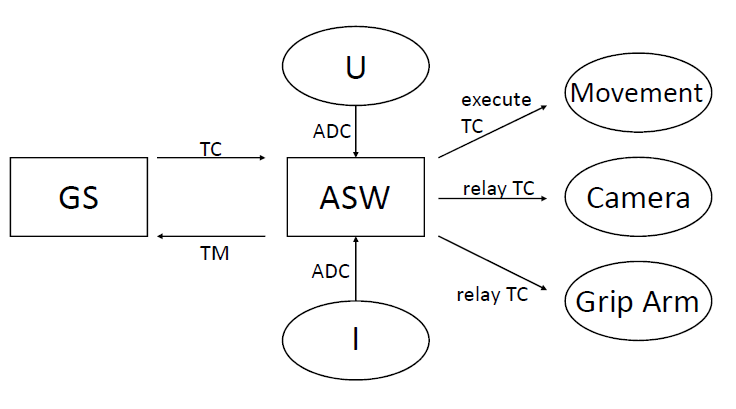
\includegraphics[scale=0.7]{system.PNG}
\caption{Functionality of the system.}
\label{fig:system}
\end{figure}


The requirements for the ASW are grouped according to its main functions. Four parts have been identified:
\begin{itemize}
\item Modes
\item Initialization
\item Commands
\item Telemetry
\end{itemize}

Modes is responsible for controlling the transitions between the different modes that the ASW has. The initialization sets up the system after its start. Commands includes receiving and executing/relaying of the received commands from the ground station. Telemetry is responsible for monitoring the system and sending a telemetry message.


\section{Function and Purpose}
The ASW shall be able to receive commands from the ground station. Those commands have to be split in the parts concerning the movement, the grip arm and the camera. Commands for the movement shall be executed, while commands for the other two devices are passed on to separate controllers. Additionally, the ASW shall monitor the voltage of the battery and the current taken by the motor. The battery voltage shall be included in a telemetry set, sent back to the ground station.\\


\section{Constraints}

The development of the ASW is mainly constrained by the fact, that the entire hardware interacting with the SW is already chosen and present. Additionally, the other software parts controlling the rover movements, the grip arm and the camera are already implemented as well as the ground station. For that reason, the developed ASW has to be highly orientated towards those existing parts as no changes are possible in the surrounding systems anymore.

\chapter{Specific Requirements}

\section{General}

The requirements will be presented categorized in sections depending on the functionality or the ASW part that shall apply them. Under each section all the requirements are listed, and for a better understanding of the system and better reference to the requirement a global numbering system has been prepared.\\

Each requirement number has the numbering form of "RXX-XX": "R" for requirement followed by four numbers separated by a dash. The first two numbers refer to the group/section each requirement belongs, while the two other numbers are the number of the requirement in the group.\\

Section/group list with the corresponding numbering:
\begin{enumerate}
\item[00] Modes
\item[01] Initialization
\item[02] Commands
\item[03] Telemetry
\item[04] Performance
\item[05] Interface
\item[06] Operation
\item[07] Resource
\item[08] Verification
\item[09] Acceptance testing
\item[10] Documentation
\item[11] Security
\item[12] Portability
\item[13] Quality
\item[14] Reliability
\item[15] Maintainability
\item[16] Safety
\item[17] SW Design and Programming
\end{enumerate}

As the developed ASW is highly constrained by the interacting systems, all following requirements are ranked as essential.

\section{Functional requirements}

\subsection{Modes}

The ASW shall have three different modes. Those modes are INIT, NORMAL and SAFE. The transitions between the modes are shown in \abb{fig:modes}.\\


\begin{figure}
\centering
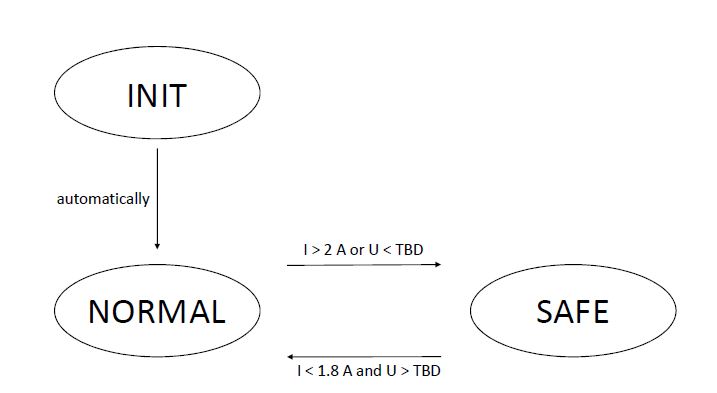
\includegraphics[scale=0.8]{modes.PNG}
\caption{Transitions between modes.}
\label{fig:modes}
\end{figure}

\textbf{R00-01}\\
The software shall have three modes: INIT, NORMAL, SAFE.\\

\textbf{R00-02}\\
The software shall start in INIT mode.\\

\newpage

\textbf{R00-03}\\
The NORMAL mode shall be reached automatically after INIT mode has finished, that means all necessary initializations are completed.\\

\textbf{R00-04}\\
During NORMAL mode telecommands are processed, telemetry is sent and the power status is monitored.\\

\textbf{R00-05}\\
If the battery voltage is lower than TBD or the current of the motor is higher than 2 A, the system shall change to SAFE mode. (TBD will be solved by the customer during SRR)\\

\textbf{R00-06}\\
In SAFE mode, all movements are stopped. The only action by the system in this case, is monitoring the power status.\\

\textbf{R00-07}\\
The system changes from SAFE to NORMAL mode, if the current of the motor is smaller than 1.8 A and the battery voltage is higher than TBD. (TBD will be solved by the customer during SRR)\\

\subsection{Initialization}

\textbf{R01-01}\\
The initialization of the software shall be done first after the start.\\

\textbf{R01-02}\\
The initialization sets up the interfaces according to the used communication busses.\\

\textbf{R01-03}\\
The initialization sets up the used hardware.

\subsection{Commands}

Specific requirements regarding the commands the ASW will receive from the ground station or equivalent controlling software.\\

\textbf{R02-01}\\
The ASW shall be able to process commands arriving at a minimum interval of 0.5 s.\\

%\textbf{R02-02}\\
%The ASW will receive the commands using a NMEA-like style of sentence. \\

\newpage

\textbf{R02-02}\\
The TC that the ASW can process shall always have the same structure as a NULL-terminated string in the format of:\\

\$ROVER,<RA>,<RD>,<RS>,<CH>,<CV>,<GAC<,<GAH>,<GAV>*<CHK><NULL> \\

\textbf{R02-03}\\
All numbers but Rover direction (<RD>) shall be ASCII-coded integer in the interval 0-100.\\

Detailed description of the command:\\

%\textbf{R02-05}\\
\textit{<RA>, Rover Angle}. Shall have a value between 0-100, being 0 the leftmost angle, 50 the 'center' angle and 100 the rightmost angle.\\

%\textbf{R02-06}\\
\textit{<RD>, Rover Direction}. Shall have a value of 0 or 1. 0 is forward movement and 1 is backward movement.\\

%\textbf{R02-07}\\
\textit{<RS>, Rover Speed}. Shall have a value between 0-100, being 0 no speed and 100 the fastest speed.\\

%\textbf{R02-08}\\
\textit{<CH>, Camera Horizontal}. Shall be the relay value through the I2C-bus.\\

%\textbf{R02-09}\\
\textit{<CV>, Camera Vertical}. Shall be the relay value through the I2C-bus.\\

%\textbf{R02-10}\\
\textit{<GAC>, Griparm Claw}. Shall be the relay value through the I2C-bus.\\

%\textbf{R02-11}\\
\textit{<GAH>, Griparm Horizontal}. Shall be the relay value through the I2C-bus.\\

%\textbf{R02-12}\\
\textit{<GAV>, Griparm Vertical}. Shall be the relay value through the I2C-bus.\\

%\textbf{R02-13}\\
\textit{<CHK>, Checksum}. Shall be an ASCII-coded hexadecimal number with byte wise XOR on preceding bytes.\\

\textbf{R02-04}\\
All commands which are not following the specified format will be ignored by the ASW.\\

\textbf{R02-05}\\
All received commands are checked for correctness by the ASW using the checksum.\\

\subsection{Telemetry}

The telemetry section includes all monitoring tasks as well as the information sent to the ground station.\\

\textbf{R03-01}\\
The ASW shall be able to monitor the battery voltage every 0.25 s via the ADC.\\

\textbf{R03-02}\\
The ASW shall be able to monitor the current of the motor every 0.25 s via the ADC.\\

\textbf{R03-03}\\
The ASW shall send telemetry every 0.5 s.\\

\textbf{R03-04}\\
The sent TM shall always have the same structure as a NULL-terminated string in the format of:\\

\$ROVERGS,<Battery Voltage>*<CHK><NULL>\\

Detailed description of the telemetry values:\\

%\textbf{R03-04}\\
\textit{<Battery Voltage>}. Shall be a float value with one decimal number.\\

%\textbf{R03-05}\\
\textit{<CHK>, Checksum}. Shall be an ASCII-coded hexadecimal number with byte wise XOR on preceding bytes.\\


\section{Performance requirements}

\textbf{R04-01}\\
Every command shall be executed before the next one arrives setting the deadline to the minimum interval of arriving commands (see R02-01 for the value).\\

\section{Interface requirements}

\textbf{R05-01}\\
Communication between the terminal and the rover shall be done via UART protocol.\\

\newpage

\textbf{R05-02}\\
Communication between the ASW and the steering units of the camera and the grip arm shall be made via I2C protocol.\\

\section{Operational requirements}
None.

\section{Resource requirements}
None.

\section{Verification requirements}
None.

\section{Acceptance testing requirements}
None.

\section{Documentation requirements}
None.

\section{Security requirements}
None.

\section{Portability requirements}
None.

\section{Quality requirements}
None.

\section{Reliability requirements}
None.

\section{Maintainability requirements}
None.

\section{Safety requirements}
None.

\section {SW Design and Programming Requirements}

\textbf{R17-01}\\
The ASW shall be written in C language.\\

\textbf{R17-02}\\
The code shall follow the rules dictated by the standard designed for a small software project "C-standard for Balloon Project", by Benedikt Reihs and Roger Gutierrez [4].\\

\textbf{R17-03}\\
FreeRTOS shall be used as an operating system.\\

\textbf{R17-04}\\
The ASW shall be designed according to the ESA HOOD method.\\





%--------------------------------------------------------
%
% Literaturverzeichnis
%
%-------------------------------------------------------
%	\addcontentsline{toc}{chapter}{Bibliography}
%  \bibliographystyle{abbrv}
%  \bibliography{literatur}
%-------------------------------------------------------
%
% Anhang
%
%-------------------------------------------------------
%	\begin{appendix}
%  	\chapter{Experimental Data}
\label{appdat}

%	\end{appendix}
%--------------------------------	
\end{document}
%--------------------------------


